\setchapterstyle{kao}
\setchapterpreamble[u]{\margintoc}

\todo{increase main text width (read in kao docu)}


\chapter{Standard Model Background Simulation and Data Processing}
\labch{simulation_and_processing}

The analysis presented in this thesis is highly dependent on an efficient event selection to reduce the raw IceCube trigger data to a usable atmospheric neutrino sample and on a precise estimation of both expected SM background and BSM signal events through MC simulations. This chapter describes the current simulation and event selection chain used for state-of-the-art IceCube neutrino oscillation measurements like \sidecite[0.3cm]{OVS_PRD}. The whole chain can be broadly split into 4 steps:

\begin{enumerate}[wide]
    
    \item[]{\textbf{Step 1 Event Generation:}} The initial step for all particle (non-noise) simulation is the generation of events using chosen initial distributions and fluxes. Events are usually the primary particle and the particles produced in the interaction with the ice.
    \vspace{0.2cm} 

    \item[]{\textbf{Step 2 Detector Simulation:}} The particles from the first step are propagated through the ice, producing Cherenkov photons, which are then propagated further until they reach a DOM or are absorbed. If they hit a DOM the detector response (accepatance and PMT) is simulated.
    \vspace{0.2cm} 
        
    \item[]{\textbf{Step 3 Processing:}} Starting from the PMT output, both real data and simulation are processed through the in-ice trigger, the online filter and processing, and the low energy event selection to produce a neutrino dominated sample.
    \vspace{0.2cm} 

    \item[]{\textbf{Step 4 Reconstruction:}} FLERCNN bliblablub
    
    \todo{add short description of the reconstruction (L6 to final?)}

\end{enumerate}

This chapter only describes the event generation for the SM background simulation (neutrinos and muons), while the signal simulation is described in \refch{signal_simulation}. The detector simulation is identical for both signal and background events while processing and reconstruction are applied to all simulation and data in the same way. Splitting the simulation steps has the advantage of reusing the outputs of for example the generation step to propagate the particles with different ice model, in order to estimate the systematic impacts of uncertainties of the ice properties. Similar approach can be taken for varying detector response and through this a more efficient (reduced) use of computing resources can be achieved. The following sections describe the different steps in more detail and the last section, \refsec{systematic_uncertainties}, describes the related systematic uncertainties considered for this work.


\section{Event Generation} \labch{sm_event_generation}

The MC is used in the analysis by applying a method called \textit{forward folding}, where a very large number of events (signal and background) is produced using sampling distribution that are tuned to have a large selection efficiency. Those distributions don't have to be physically correct distributions, but they need to cover the full parameter space of interest for the analysis. To produce the correct physical distributions each event gets a weight, which can be used to estimate the expected number of events given a specific choice of physics and nuisance parameters. The large number of raw MC events ensures a good estimation of the expected numbers and weighted distributions. 

The analysis itself is then performed by comparing the weighted MC distributions to the observed data. This is done by binning them as will be described in \refch{analysis} and calculating a loss function comparing the bin expectations to the data. By varying the physics and nuisance parameters, that govern the weights, the loss function can be minimized and the parameters producing MC that describes the data best are found. In order to achieve a reliable result with this method the MC needs to be precise and as close to the data as possible (at least at the final selection step). 


\subsection{Neutrinos}

Due to the very low interaction rate of neutrinos, the event generation is performed in a way that forces every event to interact in a chosen sampling volume. The weight of each event is then calculated as the inverse of the simulated neutrino fluence
\begin{equation}
    w = \frac{1}{F_{\mathrm{sim}}} \frac{1}{N_{\mathrm{sim}}}
    \;,
    \labeq{neutrino_generation_weight}
\end{equation}
where $F_{\rm{sim}}$ is the number of neutrino events per energy, time, area, and solid angle and $N_{\rm{sim}}$ is the number of simulated events. If this weight is multiplied by the livetime and the theoretically expected neutrino flux for a given physical model, it results in the number of events that this event would produce. The used baseline neutrino flux computed for the South Pole is taken from \sidecite{PhysRevD.92.023004_Honda_Flux}.

The chosen simulation volume is a cylinder centered in DeepCore with radius and height chosen such that all events possibly producing a signal are contained. The different sizes are chosen depending on energy and neutrino flavor are shown in \reftab{genie_sampling_cylinder}.
\begin{table}[h]
    \begin{center}
        \small
        \begin{tabular}{ p{1.0cm} p{1.8cm} p{1.3cm} p{1.3cm} p{1.4cm} p{0.6cm} }

            \hline\hline

            \textbf{Flavor} & \textbf{Energy [\si{\giga\electronvolt}]} & \textbf{Radius [\si{\metre}]} & \textbf{Length [\si{\metre}]} & \textbf{Events/File}  & \textbf{Files}\\ 

            \hline\hline

            \multirow{4}{*}[-1.em]{ $\nu_e+\bar{\nu_e}$ }
            & 1-4
            & \multirow{1}{*}[-1.em]{ 250 }
            & \multirow{1}{*}[-1.em]{ 500 }
            & 450000
            & \multirow{4}{*}[-1.em] {650} \\

            \cmidrule{2-2}
            \cmidrule{5-5}
            
            & 4-12
            & 
            & 
            & \multirow{1}{*}[-1.em] { 100000 }
            & \\

            \cmidrule{2-4}

            & 12-100
            & 350
            & 600
            & 
            & \\

            \cmidrule{2-5}

            & 100-10000
            & 550
            & 1000
            & 57500
            & \\

            \hline
            \hline

            \multirow{4}{*}[-1.em]{ $\nu_\mu+\bar{\nu_\mu}$ }
            & 1-5
            & 250
            & 500
            & 408000
            & \multirow{4}{*}[-1.em] {1550} \\

            \cmidrule{2-5}
            
            & 5-80
            & 400
            & 900
            & 440000
            & \\

            \cmidrule{2-5}

            & 80-1000
            & 450
            & \multirow{1}{*}[-1.em] { 1500 }
            & 57500
            & \\

            \cmidrule{2-3}
            \cmidrule{5-5}

            & 1000-10000
            & 550
            &
            & 6700
            & \\

            \hline
            \hline

            \multirow{4}{*}[-1.em]{ $\nu_\tau+\bar{\nu_\tau}$ }
            & 1-4
            & \multirow{1}{*}[-1.em]{ 250 }
            & \multirow{1}{*}[-1.em]{ 500 }
            & 1500000
            & \multirow{4}{*}[-1.75em] {350} \\

            \cmidrule{2-2}
            \cmidrule{5-5}
            
            & 4-10
            & 
            & 
            & 300000
            & \\

            \cmidrule{2-5}

            & 10-50
            & 350
            & 600
            & 375000
            & \\

            \cmidrule{2-5}

            & 50-1000
            & 450
            & 800
            & 200000
            & \\

            \cmidrule{2-5}

            & 1000-10000
            & 550
            & 1500
            & 26000
            & \\

            \hline

        \end{tabular}
    \end{center}
    \caption[GENIE generation cylinder volumes]{Cylinder volumes used for GENIE neutrino simulation generation. Cylinder is always centered in DeepCore at $(x,y,z) = (46.29,-34.88,-330.00)$ \si{\metre}.}\labtab{genie_sampling_cylinder}
\end{table}
The directions of the neutrinos are sampled isotropically in zenith and azimuth and the energies are sampled from a power law $E^{-2}$. The number of simulated events is chosen such that the livetime is more than \SI{70}{years} for each flavor. Neutrinos and antineutrinos are simulated with ratios of 70\% and 30\%, respectively.

To simulate the neutrino interaction with the ice the \textsc{Genie} event generator \sidecite{genie} is used resulting in the secondary particles and the kinematic and cross-section parameters. Muons produced in these interactions are propagated using \textsc{Proposal} \sidecite{proposal}, also simulating their Cherenkov light output. The shower development of gamma rays, electrons, and positrons below \SI{100}{\mega\electronvolt} and hadronic showers below \SI{30}{\giga\electronvolt} is simulated using \textsc{Geant4} \sidecite{geant4} while for higher energies an analytical approximation from \sidecite{raedel_wiebusch_cherenkov_yield} is used.


\subsection{Muons}

Atmospheric muons are generated on a cylinder surface enclosing the full IceCube detector array. The cylinder has a height of \SI{1600}{\meter} and a radius of \SI{800}{\meter}. The energy is sampled from an $E^{-3}$ power law while the other sampling distributions (position, direction) are found from parameterizations based on \sidecite{muon_parameterization}. This work uses full \textsc{Corsika} \sidecite{corsika} simulations of muons to tailor the parameterizations, starting from cosmic ray interactions with atmospheric nuclei using the cosmic ray flux model from \sidecite{gaisser_cosmic_ray} and producing the muons applying the hadronic interaction model SIBYLL 2.1 \sidecite{sibyll_hadronic}. After the generation, they are propagated through the ice with PROPOSAL producing photons, treating them exactly like the muons produced in neutrino interactions.

Since the offline processing and selection steps described in \refsec{offline_filter} and \refsec{reconstruction} reduce the muon contamination to a negligible level, it is difficult to correctly estimate the expected number of muon events at final selection level and therefore two separate sets of muon simulation are produced. \textbf{A first set} including all events resulting from the above described generation to tune the lower level selection (up to L4) and \textbf{a second set} to estimate the muon contamination at higher levels (above L5), which only accepts muon events if they pass through a smaller cylinder centered in DeepCore (height of \SI{400}{\meter} and radius of \SI{180}{\meter}) and rejects events based on a KDE estimated muon density at L5 (in energy and zenith) increasing the simulation efficiency at L5 significantly \todo{put a number on this significant increase?}.


\section{Detector Simulation}

The detector simulation is performed after the event generation, where the initial particles and the resulting photons and secondary particles from their propagation were produced. This part of the simulation chain is applied to all particle simulation, both neutrino and muon generation explained in \refch{sm_event_generation}, but also the particles from the HNL signal generation explained in detail in \refch{signal_simulation}. The detector simulation can be split into two parts, the propagation of the photons and the simulation of the detector response (including internal noise).


\subsection{Photon Propagation}

For any Cherenkov detector, but especially for ice-Cherenkov detectors, like IceCube, the propagation of the photons is a crucial part of the detector simulation. Any photon that was produced in the event generation is individually traced through the ice, simulating scattering and absorption processes, taking into account the local ice properties, estimated with a chosen ice model. The propagation is done using \textsc{clsim} \cite{clsim} which is an implementation of the \textit{Photon Propagation Code (\textsc{PPC})} \sidecite{ppc} in \textsc{OpenCL}. It is optimized to be run very efficiently on GPUs, which is what is done for IceCube simulation production. The ice is modeled as a set of \SI{10}{\meter} thick, almost horizontal layers with specific absorption and scattering lengths. The \textit{South Pole ICE (SPICE)} model \sidecite{spice_ice_model} accounts for the layers being tilted by a small amount (\todo{put a number on the tilt angle?}) and the absorption and scattering lengths having a non-uniformity with respect to the azimuth direction. \todo{add plot with ice scattering/absorption lengths used for simulation} \reffig{simulation_ice_model} shows the values of this model for the different depths, indicating the location of IceCube, DeepCore, and the dust layer. 


In an initial step, each photon's absorption length is sampled from an exponential distribution with the expectation value at the current layer's absorption length. The following propagation steps are performed in parallel for all photons. In each of those steps, corresponding to a single scattering event, the photon travels a length that is sampled from an exponential distribution with the expectation value at the scattering length of the current layer and the scattering angle chosen based on a combination of a simplified Mie scattering distribution \sidecite{mie_scattering} and a Henyey-Greenstein distribution \sidecite{henyey_greenstein}. The parameters defining the shape of these distributions were calibrated using data from \textit{in-situ} LED calibration runs. These steps are continuously repeated until each photon reached a DOM or was absorbed \sidenote{When it traveled its full absorption length, sampled in the initial step}. After all photons have been propagated in that manner, the final step is to output the photons that reached a DOM for further processing.


\subsection{Detector Responses}

The second part of simulating the IceCube detector is the DOM response itself, but not all the photons that reached a DOM are accepted as being observed. Whether a photon was detected is determined individually based on the total efficiency and the angular acceptance curve of the specific DOM. The total efficiency includes effects of the DOM glass, PMT quantum and photo-electron collection efficiencies, and it is wavelength dependent. Additionally, there is another angle dependent effect called \textit{hole ice}. This effect is due to varied ice properties resulting from the re-freezing process of the water column inside the borehole after deployment of the string. Due to bubble formation the ice is less transparent than the surrounding ice and an additional angular acceptance is added, which can increase or decrease the efficiency to detect photons. Accepted photons are converted into a so-called \textit{Monte Carlo photo-electron (MCPE)}. The amount of charge measured for each MCPE is determined by sampling from a mixture of two exponential distributions and a normal distribution. This \textit{single photo-electron (SPE)} distribution was tuned to match the observed distribution in each DOM in an \textit{in-situ} calibration study \sidecite{spe_respose_pmt}. \reffig{spe_distribution} shows the distribution compared to a lab measurement. Based on the sampled charges and times of MCPEs, the voltage waveforms for the (two) different readout channels are simulated and passed on to the trigger simulation starting with \textit{WaveDeform}, which was already mentioned in \refsec{ice_and_DOMs}.

Next to the Cherenkov photons, IceCube also observes photons that are produced in radioactive decays inside the DOMs, both in the glass housing sphere and the PMT glass itself. To simulate this internal noise, the \emph{Vuvuzela} module \sidecite{MLarson_master, MLarson_phd} is used to create additional MCPEs that are fed into the same simulation chain described above. This module takes into account thermal and non-thermal components and their times are sampled using parameterizations of the measured distributions, where the thermal noise component is uncorrelated photons and the non-thermal component is from burst of photons. The noise hits are simulated by drawing the times from a constant rate Poisson process and the number of photons from a Poisson distribution, then the time differences between the individual photons per hit is found, based on a Log-Normal distribution. The simulation is defined by 5 parameters that are calibrated for each DOM individually. \reftab{vuvuzela_parameters} shows a set of typical values for these parameters. \todo{add table with typical vuvuzela noise parameters}


\section{Processing}

After the detector simulation is performed, all MC and data are processed in exactly the same way. This section explains the trigger and event selection that is applied starting from the raw voltage measured by the PMTs. Most parts of this processing are identical to the procedure already described in \sidecite{ATrettin_phd, ELohfink_phd}. It is split in different steps run inside the ice, at the South Pole, and after the data was transferred to the North. The complexity and computational cost of the processing increases with each step, while the total number of events reduces, making it feasible and reducing the use of computational resources on events that are not of interest for the analysis. 


\subsection{Trigger and Filter}

Before the data can be sent to the North, the initial signal coming from the PMT (for data) or from the detector response simulation (for MC) is a voltage waveform, which has to be digitized and information of photon hits has to be extracted. The trigger and filter explained here are tailored to select events that passed through the DeepCore volume, while rejecting background events (either from atmospheric muons or from random noise). There are other filters used in IceCube which will not be explained here, since they are not relevant for this work. A full description of the instrumentation and the online systems can be found in \sidecite{Aartsen:2016nxy}.


\subsubsection{In-ice Trigger} \labsec{trigger}

The trigger is applied inside the DOM in the ice before sending the information to the ICL on the surface. The time dependent voltage curves are captured if a pre-defined threshold value is exceeded. Once the threshold set to the equivalent of \SI{0.25}{PE} is crossed, \SI{6.4}{\micro\second} of the waveform are coarsely digitized by a \textit{Fast Analog-to-Digital Converter (FADC)} with a sampling rate of \SI{40}{\mega\hertz} \sidecite{ABBASI2009294_data_acquisition}. Additionally, the first \SI{427}{\nano\second} are digitized using an \textit{Analog Transient Waveform Recorder (ATWD)} with a sampling rate of \SI{300}{\mega\hertz} \sidecite{ABBASI2009294_data_acquisition}, but only if some trigger condition is met, because this readout frequency is too high to be sampled directly and requires some buffering. For DeepCore, the HLC condition already mentioned in \refsec{ice_and_DOMs} has to be met for three DOMs inside the fiducial volume within a time window of \SI{5}{\micro\second}. If this is the case, all waveforms that crossed the threshold within a \SI{20}{\micro\second} time window around the trigger are digitized and sent to the ICL for further processing. This trigger is called \textit{Simple Multiplicity Trigger 3 (SMT-3)}. The DOM hits that are read out in this process, but do not meet the HLC condition, are called \textit{soft local coincidence (SLC)} hits \sidecite{ABBASI2009294_data_acquisition}. The rate of the DeepCore SMT-3 trigger is $\sim$\SI{250}{\hertz} \sidecite{2017JInst..12P3012A_Instrumentation_Systems}, accepting $\sim$\SI{70}{\percent} of $\nu_\mu$-CC events at \SI{10}{\giga\electronvolt} and $\sim$\SI{90}{\percent} at \SI{100}{\giga\electronvolt} \sidecite{DeepCore_design_Abbasi2012615}. The trigger efficiencies for different SMT triggers, including the DeepCore SMT-3, are shown in \reffig{trigger_efficiencies}. \todo{add figure with trigger efficiencies (SMT 3,4,6,8)}


\subsubsection{Online Filter} \labsec{online_filter}

The digitized waveforms are sent to the ICL, where a further filter is applied \textit{online} \sidenote{Where \textit{online} means running on hardware at the South Pole.}. First the WaveDeform algorithm is run to extract photon arrival times and charge from the waveforms, then the DeepCore filter is applied, which is an iterative hit cleaning starting from HLC hits and removing any hits outside a \SI{125}{\meter} radius and a \SI{500}{\nano\second} time window (called \textit{radius-time cleaning (RT-cleaning)}) of the initial hit. This mainly rejects unphysical SLC hits, which are potentially caused by random noise. The following selection steps are done using the resulting cleaned pulses.

Next, an additional cut is applied to reject events that are likely to be caused by atmospheric muons. This is done by splitting the hits depending on whether they were inside the DeepCore fiducial volume or outside and then calculating the speed of each hit outside the fiducial volume towards the \textit{center of gravity {COG}} of the hits inside. If one of them has a speed close to the speed of light, the whole event is rejected, because this is a strong indication for a muon event.

As input for the further selection levels, a few event properties, like vertex position and direction, are determined using fast and simple event reconstructions. After the DeepCore online filter, the rate is about \SI{15}{\hertz}, which can be sent to the North via satellite for further processing.


\subsection{Event Selection} \labsec{event_selection}

After the data was sent to the North, the \textit{offline} filters and selection are applied to further recude reduce the background of atmospheric muons and noise. The selection is split into three levels referred to as \textit{Level 3-5 (L3-L5)}, which bring down the neutrino and muon rate to $\sim$\SI{1}{\milli\hertz}, while the remaining fraction of random noise is below \SI{1}{\percent}.


\subsubsection{Level 3} \labsec{level_3}

At the first offline filtering level, Level 3, 1D cuts are used to reduce atmospheric muons, pure noise, and coincident muons. These cuts are targeting regions where the data/MC agreement is poor, so that more sophisticated \textit{machine learning (ML)} techniques can be applied at later levels. The cuts are made using 12 control variables, that are inexpensive to compute for the very large sample at this stage. The variables are related to position, time, and overall number of hits in the event.

Pure noise hits, that are temporally uncorrelated, are cleaned by applying a \SI{300}{\nano\second} sliding window, requiring the containment of more than 2 hits at its maximum. Additionally, an algorithm is run to check whether the hits show some directionality, accepting them only if they do.

To reduce the amount of muons a series of cuts is applied using spatial and temporal information. Events that have more than 9 hits observed above \SI{-200}{\meter} or the first HLC hit above \SI{-120}{\meter} are rejected as well as events where the fraction of hits in the first \SI{600}{\nano\second} of the event is above 0.37, ignoring the first two hit DOMs. Additionally, the ratio between hits in the veto region and the DeepCore fiducial volume is required to be below 1.5.

If a muon enters the detector after the data acquisition was already triggered, it causes events that span over a much larger time range. To reduce those coincident events, the time difference between first and last pulse cannot be above \SI{5000}{\nano\second}. This cut mainly affects a region of very poor data to MC agreement, because coincident events are not simulated at all.

The L3 cuts remove \SI{95}{\percent} of the atmospheric muons and >\SI{99}{\percent} of pure noise hits, while keeping >\SI{60}{\percent} of the neutrino events. The sample now roughly contains muons/neutrinos/noise at a ratio of 100:10:1 with a total rate of $\sim$\SI{0.5}{\hertz}.

\todo{add example plots (2?) for L3 cut variables and applied cuts}

\subsubsection{Level 4} \labsec{level_4}

After the total rate was reduced by the simple cuts of L3 and the overall agreement between data and MC is established, ML techniques can be applied to further reduce the background. For Level 4, two \textit{Boosted Decision Trees (BDTs)} \todo{reference BDT} classifier are trained to separate neutrino events from atmospheric muons and noise hits, separately. The output of each classifier, a probability score, can be seen in \reffig{level_4_classifiers}. The noise filter is applied first and an event passes the score is larger than 0.7, reducing the noise hits by a factor of 100, while keeping \SI{96}{\percent} of neutrinos. Then the second BDT classifier, trained partly on unfiltered data consisting of >\SI{99}{\percent} atmospheric muons, is applied. Rejecting events with a score smaller than 0.65 removes \SI{94}{\percent} of atmospheric muons while keeping \SI{87}{\percent} of neutrinos. This fraction varies depending on the flavor and interaction type, $\nu_\mu$-CC events for example, which have a muon in the final state, are therefore reduced to \SI{82.5}{\percent}. After applying the L4 cuts based on the BDT classifier outputs, the sample is still dominated by atmospheric muons, while the noise rate dropped to below most neutrino types.

\todo{add figure with L4 BDT classifier outputs}


\subsubsection{Level 5} \labsec{level_5}

Level 5 is the final selection level, before event reconstructions are applied. This level aims to reduce the remaining atmospheric muon rate below the rate of neutrinos. Muons not rejected by the earlier levels are those that produced little or no light in the veto regions. One possible reason is that they passed through one of the un-instrumented regions between the strings \todo{add some figure showing the corridors?} called \textit{corridors}. To reject those, special corridor cuts, based on the number of hits they produced close to a potential corridor they passed through. The potential corridor in questions is identified based on a simple infinite track fit. In addition to the corridor cuts, starting containment cuts are applied to reject events that start at the edge of the fiducial volume. Events with more than seven hits in the outermost strings of the detector or those that have a down going direction in the uppermost region are rejected. This further reduces the fraction of muons by \SI{96}{\percent} while keeping \SI{48}{\percent} of neutrinos. The rates after this level are \SI{1}{\milli\hertz} and \SI{2}{\milli\hertz} for neutrinos and muons, respectively, making it a neutrino dominated sample.

\todo{add table with rater per level (split in flavor for signal (benchmark mass/mixing?) and background)}


\section{Reconstruction} \labsec{reconstruction}

There are several methods to select and reconstruct events in IceCube.
At energies around 10-40\,GeV, where we expect the oscillation signal, the events are faint and only a few DOMs detect light.
One approach for the reconstruction of such events is described in this section.
The reconstruction uses only photons that traveled along a straight line - called \textit{direct} photons.
Using direct photons has the benefit of reducing the systematic biases caused by the large variations of the bulk ice properties; scattering and absorption.
With an average distance of 70\,m between strings in DeepCore and an effective scattering length of about 50\,m \sidecite{LUNDBERG2007619}, there will always be a fraction of direct photons arriving at the DOMs.
The used method applies a stepwise procedure, where first a cleaning routine selects events with direct photons as described in Section \refsec{hit_selection}. 
Afterward, the direction of the particle is reconstructed and finally the energy is determined as outlined in Sections \refsec{flercnn_reconstruction}.


\subsubsection{FLERCNN Event Reconstruction and Classification} \labsec{flercnn_reconstruction}

Didn't copy over SANTA/LEERA since I need the FLERCNN desciption here.


\subsubsection{Standard Model Event Morphologies}

The signals that IceCube detects vary depending on the neutrino flavor and interaction type of the event.
The two main signatures that can be observed are track-like and cascade-like events.
The observed Cherenkov light is produced by the secondary particles originating from the neutrino interactions described in Section \refsec{neutrino_interactions}.
Table \reftab{interactions_vs_signatures} shows an overview of the possible event signatures.
Minimum ionizing muons can travel for long distances and are seen as extended light signatures called tracks.
Muons can come from $\nu_\mu$-CC interactions or from $\nu_\tau$-CC followed by the decay of the $\tau$ to a muon.
However, the $\tau$ only decays to a muon with a branching ratio of BR=\SI{17}{\percent}.

Cascades are the light signal produced by the EM/hadronic showers described in Section \refsec{energy_loss}.
They come from $\nu_e$-CC and most of the $\nu_\tau$-CC interactions because the electron and the tau lose all their energy quickly and only travel a short distance.
They are also produced in all $\nu$-NC interactions since only the hadronic shower is observable and the produced neutrino escapes unseen.
The cascades at the energies considered in this work have a smaller radius than the spacing of the DOMs and are therefore seen as point-like light emitters.

% \begin{table}[h]
%     \small
%     \begin{center}
%         \begin{tabular}{  m{2.3cm} m{2.3cm} m{4.5cm} m{3.5cm}  } 
%             \hline\hline
%             \textbf{Interaction} & \multicolumn{2}{c}{\textbf{Secondary particles}} &\textbf{Signature} \\ 
%             \hline\hline
%             \multirow{2}{*}[-1.5em]{CC $\overset{\scriptscriptstyle(-)}{\nu_\mu}$ }
%             & 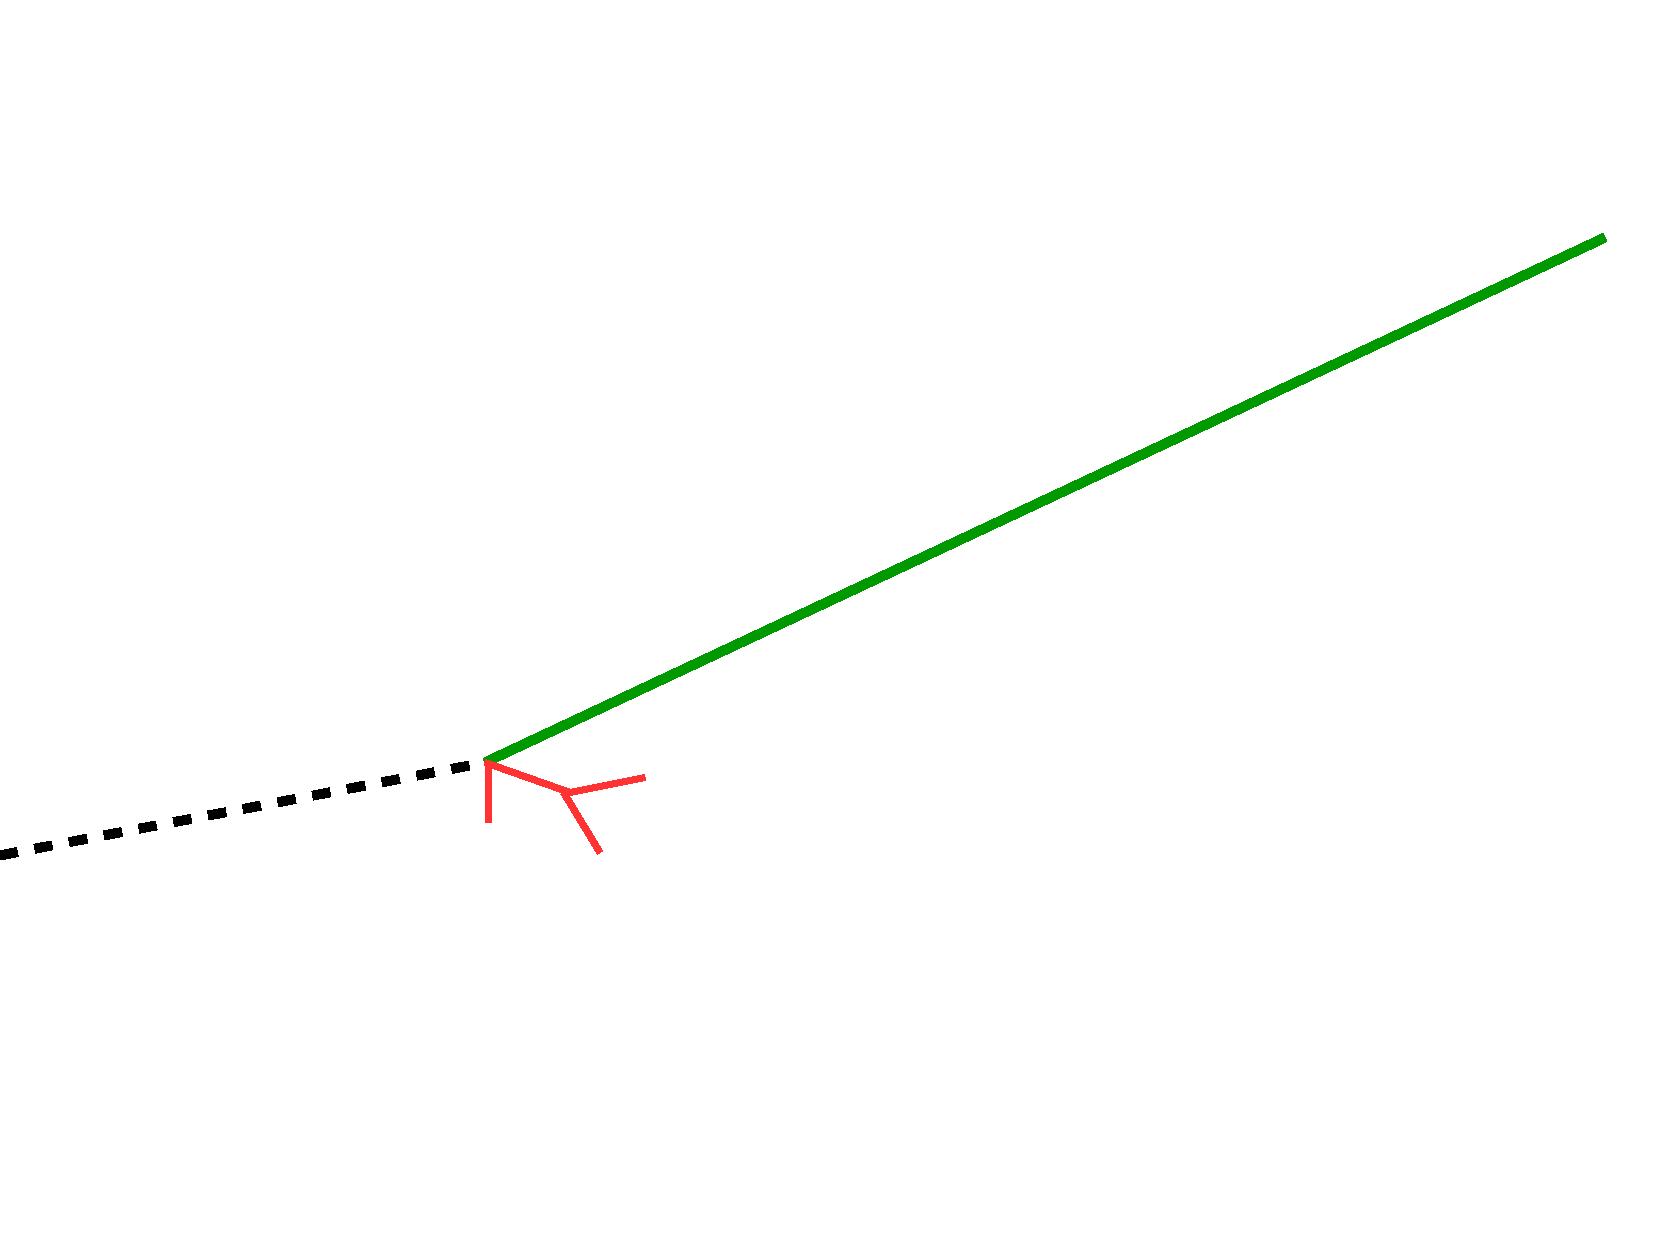
\includegraphics[width=2cm]{figures/neutrinos_properties/interaction_schematics/numu_CC_muon_only.pdf}
%             & $\mu^\pm$ track 
%             & Track-only  \\
%             \cmidrule{2-4} 
%             &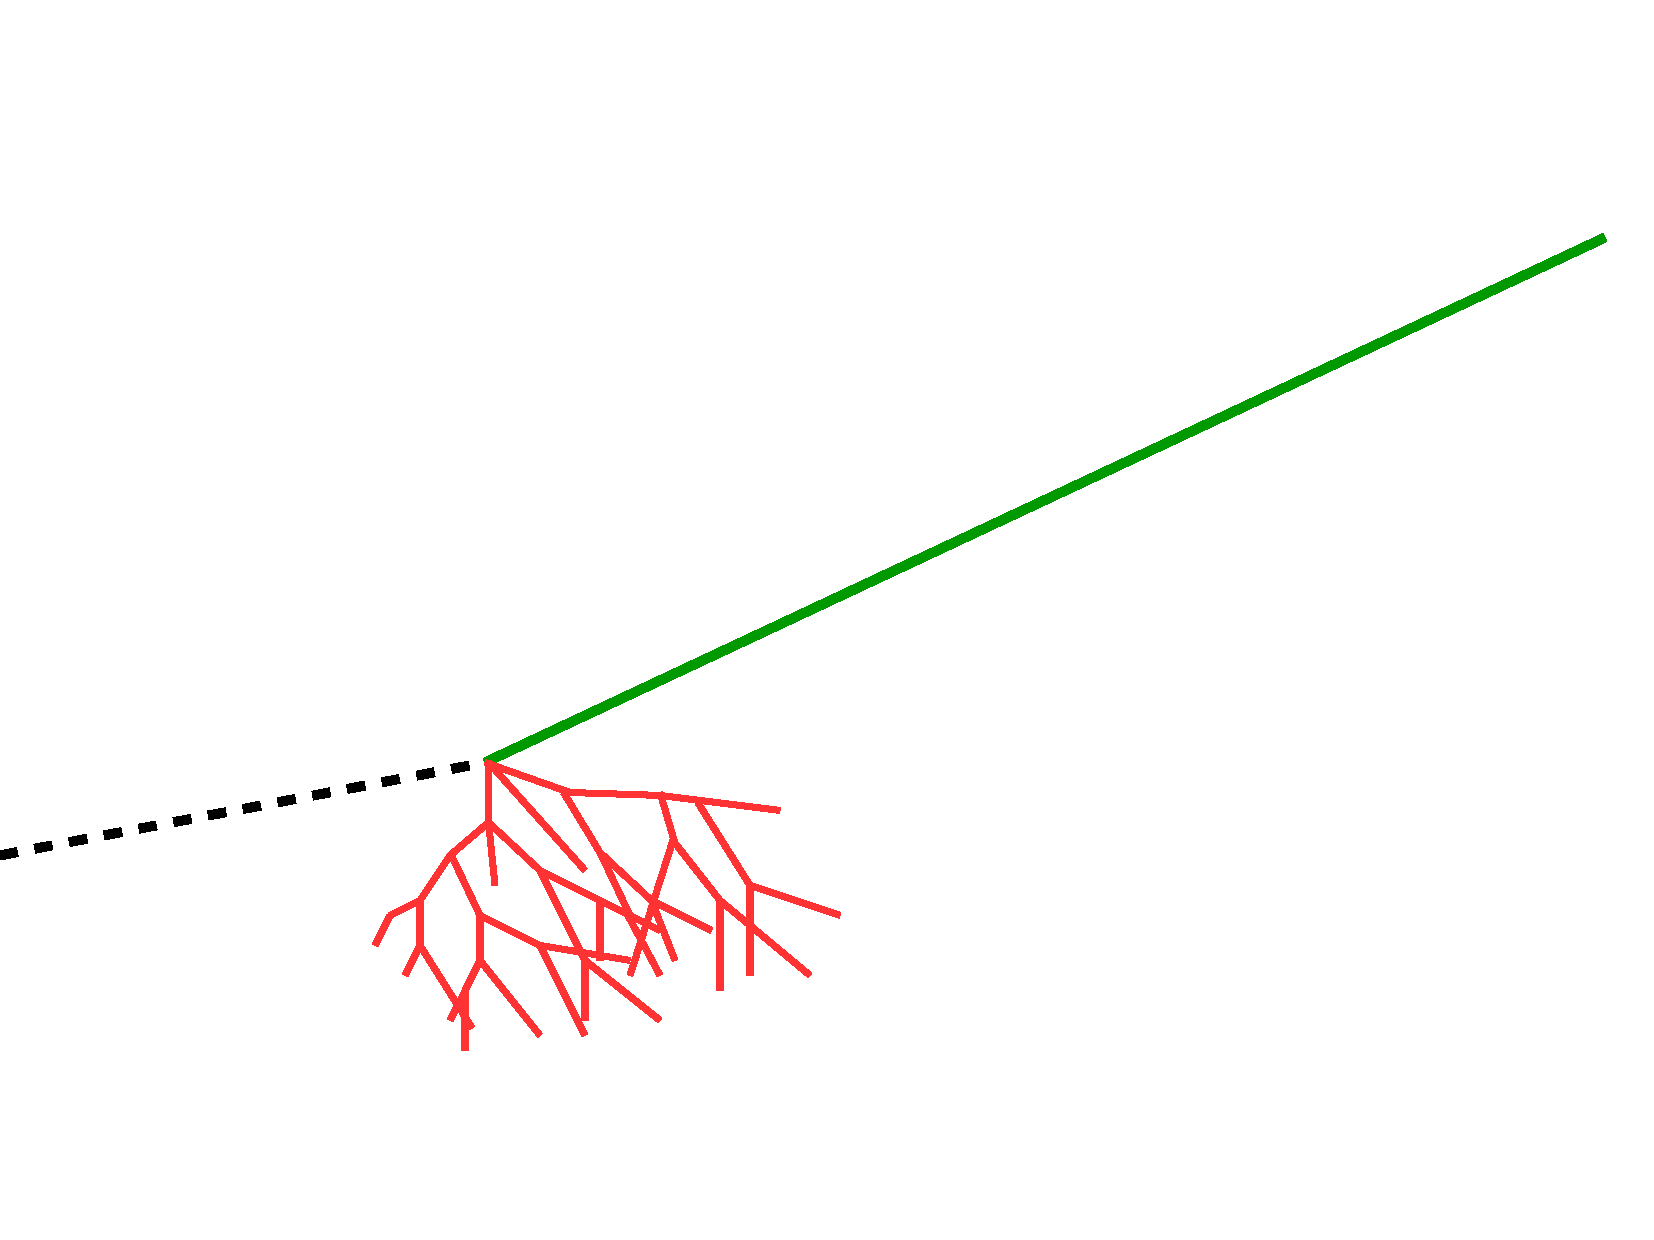
\includegraphics[width=2cm]{figures/neutrinos_properties/interaction_schematics/numu_CC_track_cascade.pdf}  
%             & $\mu^\pm$ track and hadrons 
%             & \multirow{2}{*}[-2em]{Track with cascade} \\
%             \cmidrule{1-3}
%             \multirow{2}{*}[-1.5em]{CC $\overset{\scriptscriptstyle(-)}{\nu_\tau}$ }
%             &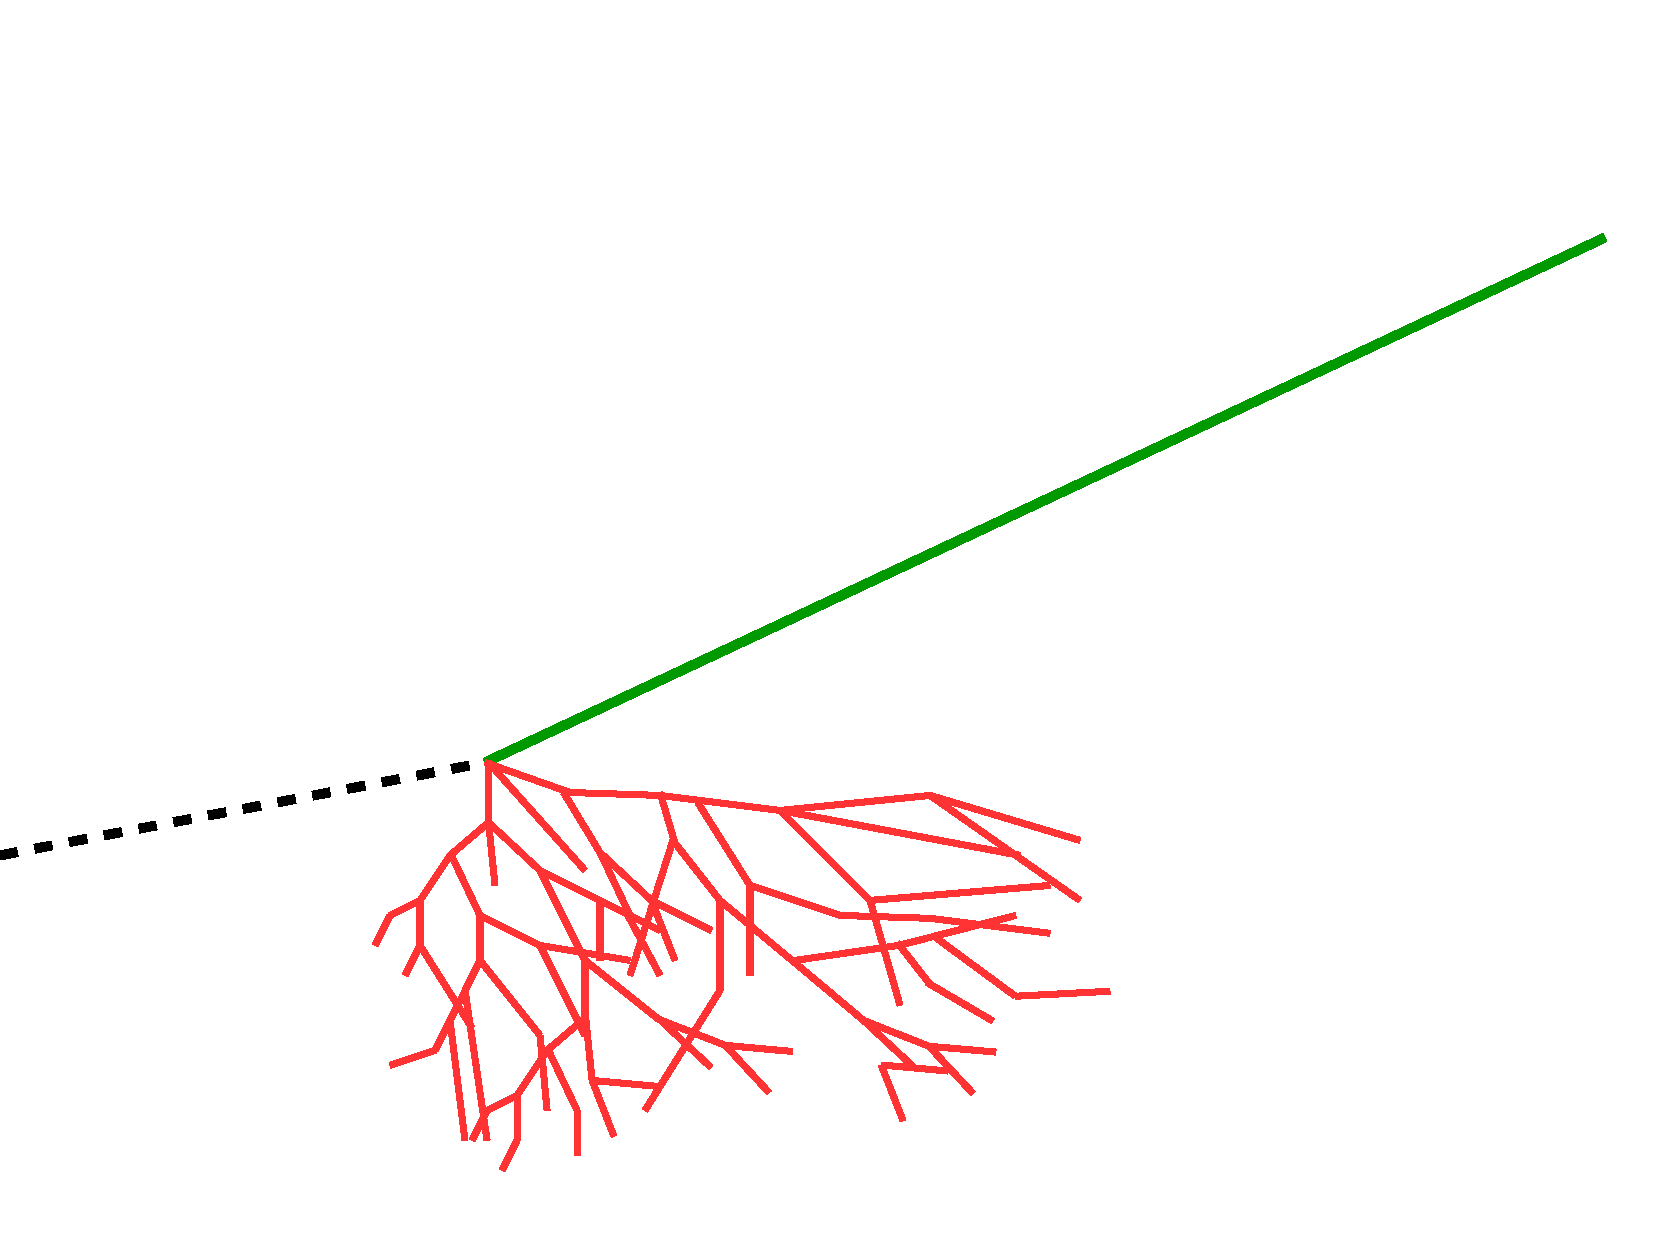
\includegraphics[width=2cm]{figures/neutrinos_properties/interaction_schematics/nutau_CC_track_cascade.pdf} 
%             & $\tau^\pm$ decaying into $\mu^\pm$ ($\sim$17\% BR), hadrons 
%             & {}\\
%             \cmidrule{2-4}
%             & 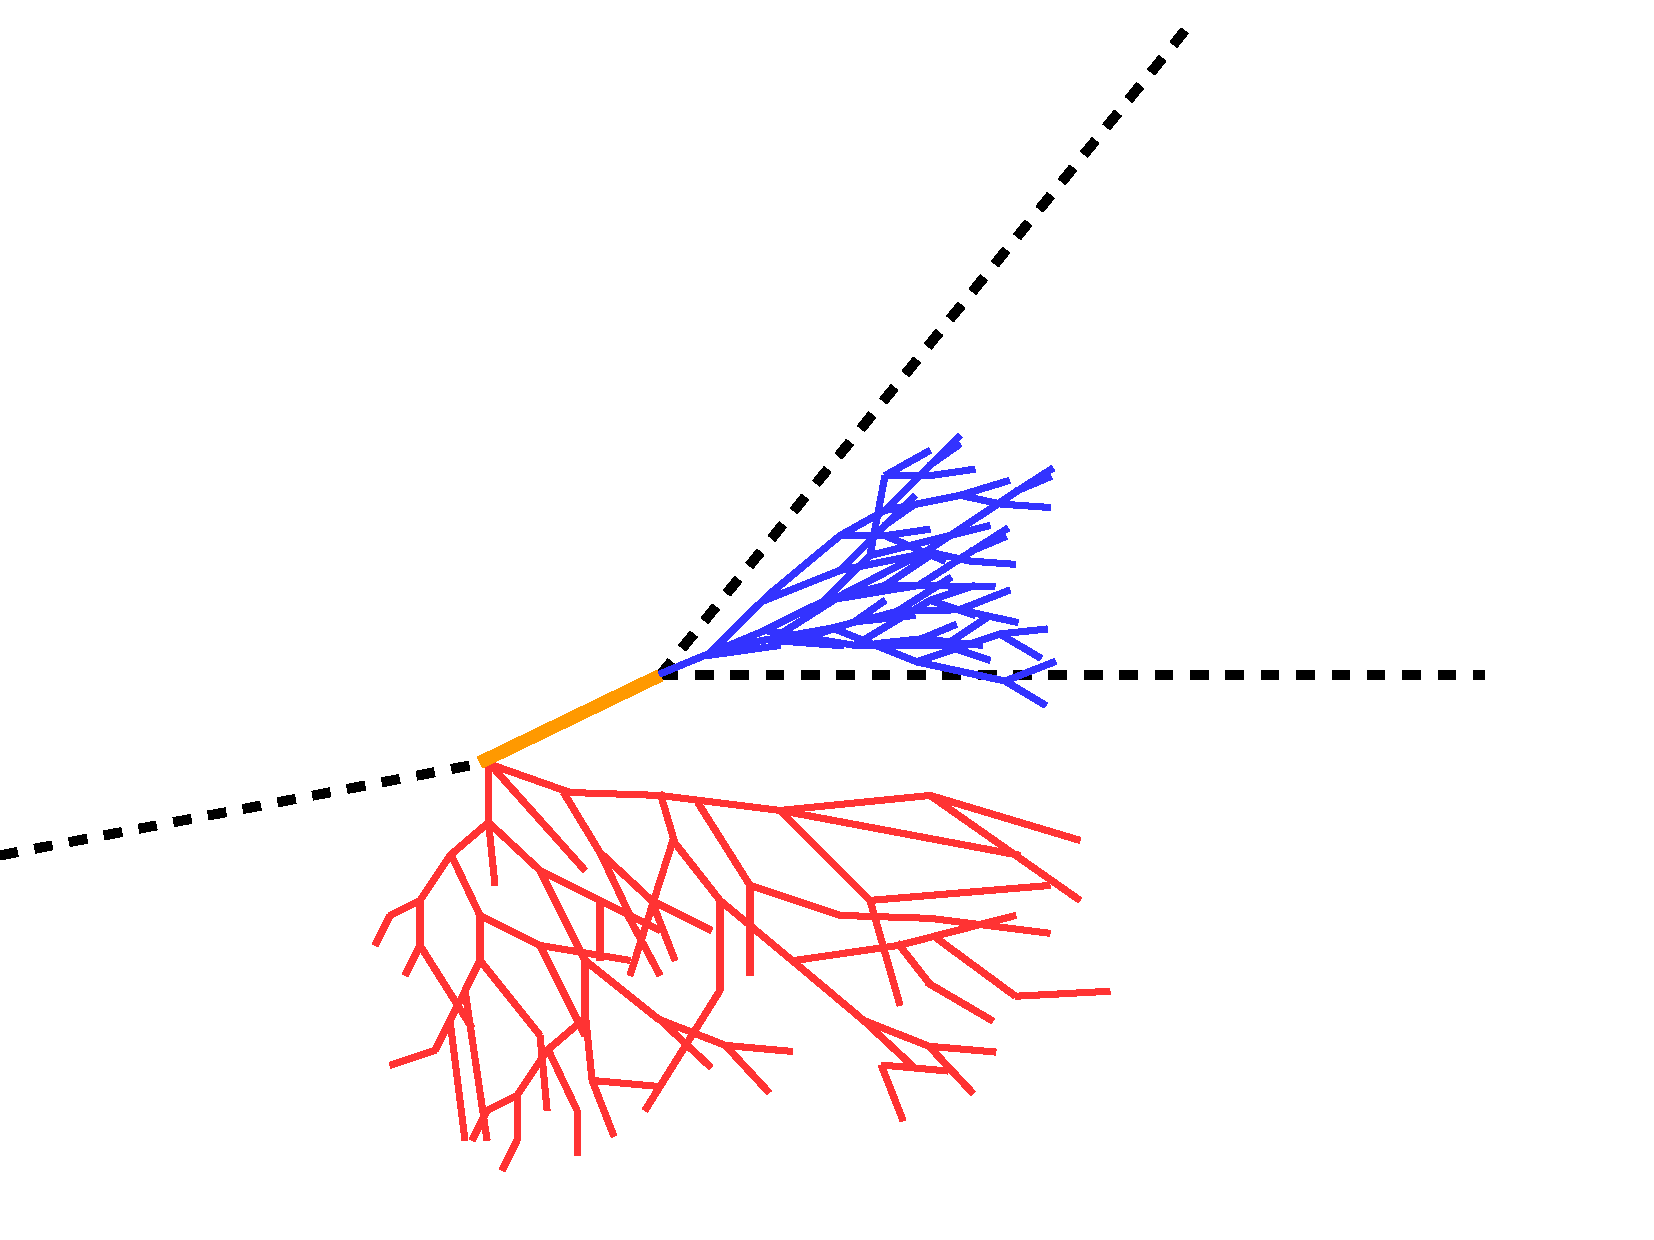
\includegraphics[width=2cm]{figures/neutrinos_properties/interaction_schematics/nutau_CC_cascadeonly.pdf}
%             & $\tau^\pm$ decaying into $e^\pm$ or hadrons ($\sim$83\% BR)  
%             & {}\\
%             \cmidrule{1-3} CC $\overset{\scriptscriptstyle(-)}{\nu_e}$ 
%             & 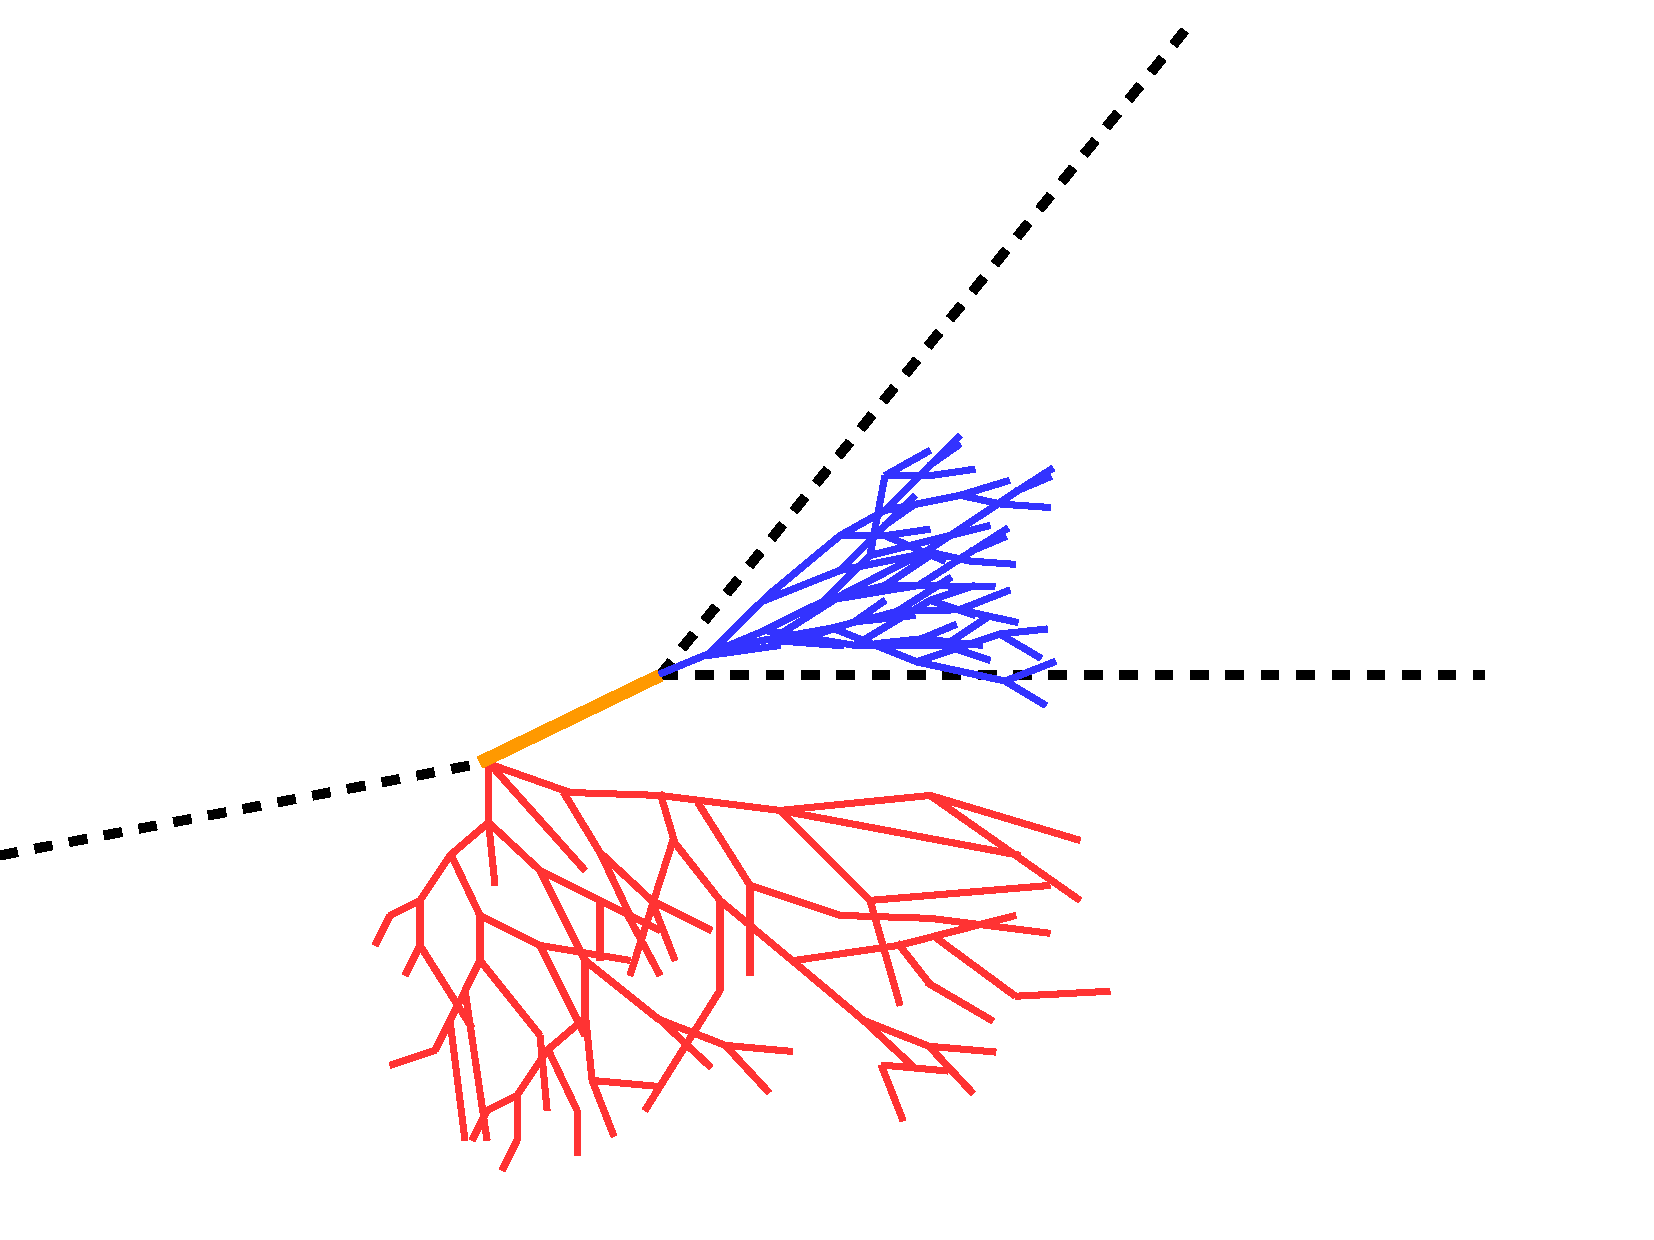
\includegraphics[width=2cm]{figures/neutrinos_properties/interaction_schematics/nue_CC_cascadeonly.pdf}
%             & $e^\pm$, hadrons & {Cascade-only}\\
%             \cmidrule{1-3}
%             NC $\overset{\scriptscriptstyle(-)}{\nu_\ell}$ 
%             & 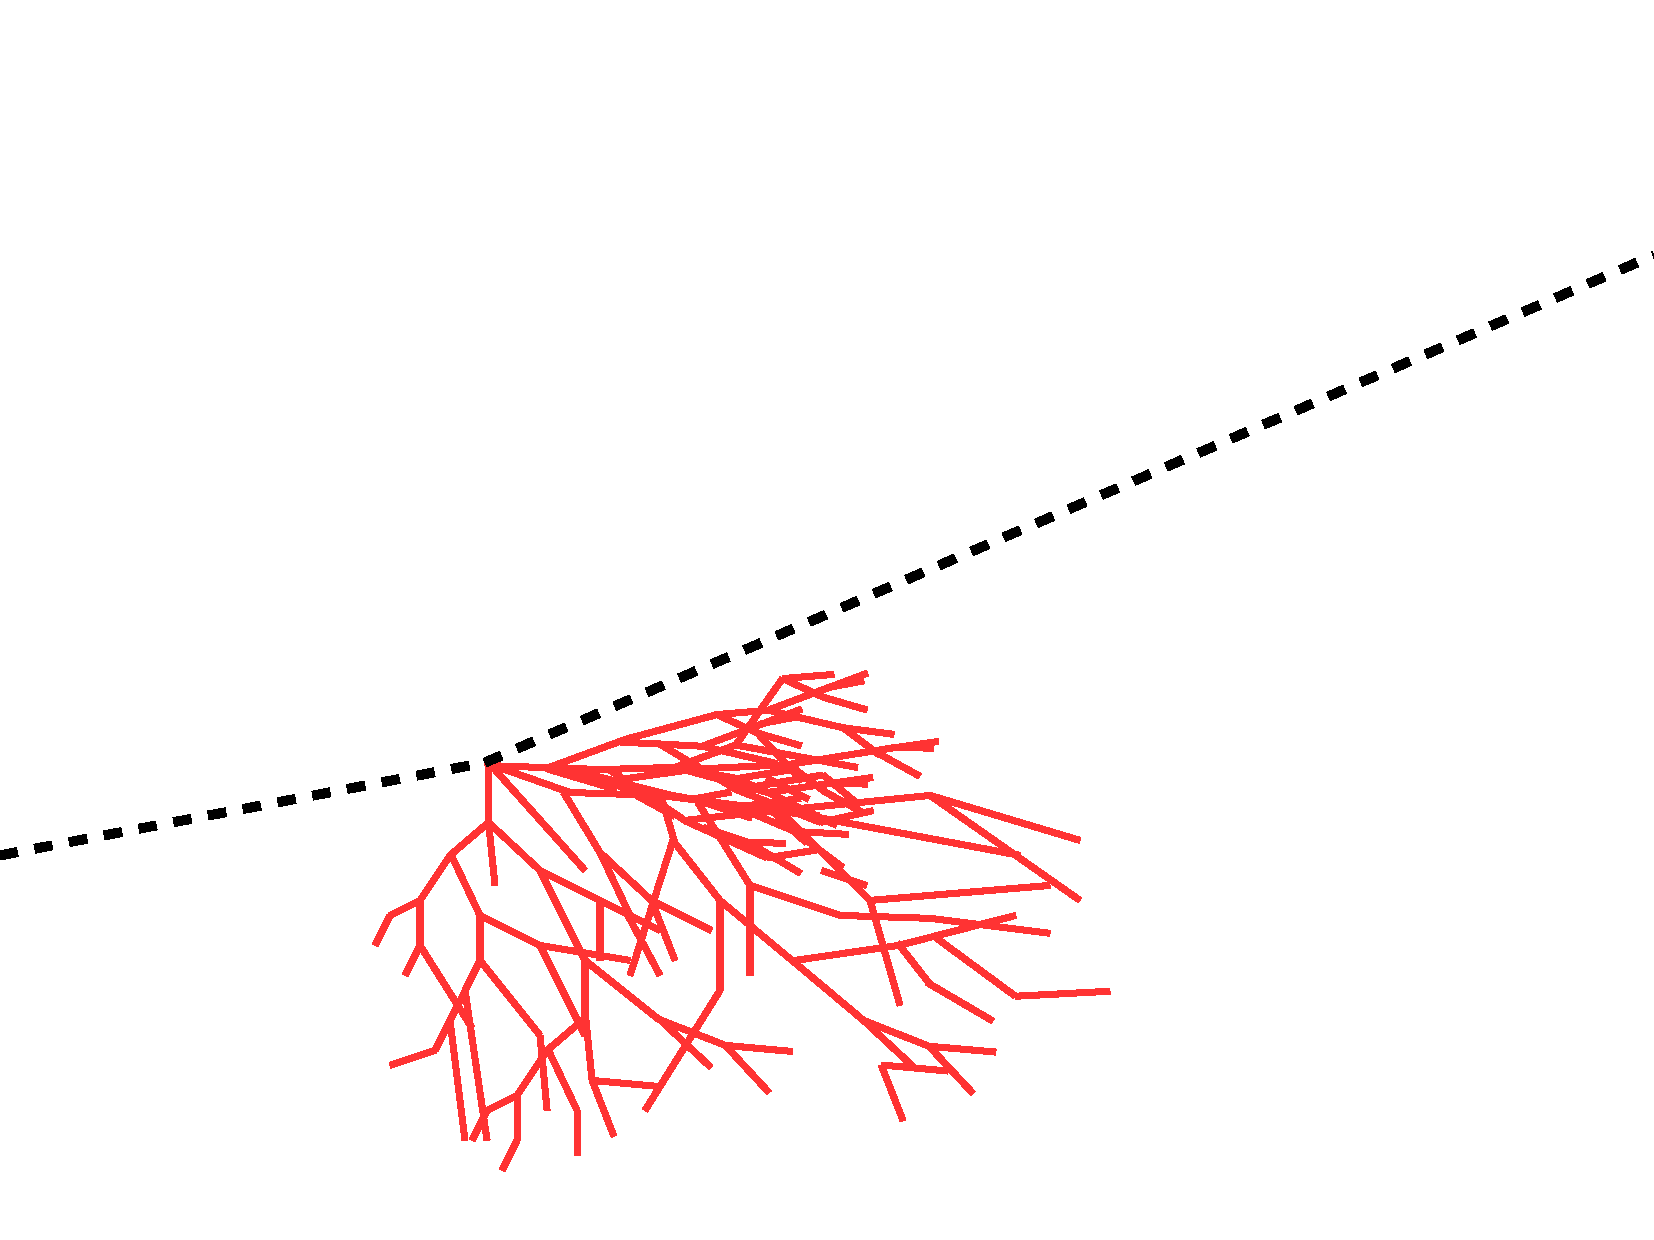
\includegraphics[width=2cm]{figures/neutrinos_properties/interaction_schematics/nuall_NC_cascadeonly.pdf} 
%             & hadrons &  {} \\
%             \hline
%         \end{tabular}
%     \end{center}
%     \caption[Event signatures in IceCube and their underlying interactions, taken from~\sidecite{ATerliuk}]{IceCube event signatures, their underlying interaction type and the particles that produce them. Also shown are the secondary particles produced in the interactions. Black dashed lines represent neutrinos, green lines muons, and blue and red lines are particles in electromagnetic and hadronic cascades, respectively. Taken from~\sidecite{ATerliuk}.}
%     \labtab{interactions_vs_signatures}
% \end{table}

The existence of the two types of event morphologies and their origins imply that by identifying track-like events we can identify events coming (mainly) from $\nu_\mu$-CC interactions and therefore obtain a flavor identification.
This is a crucial part of performing an oscillation analysis as will be further discussed in Section \refsec{analysis_principle}.

\subsubsection{Final Level Event Selection}

add this here or in the analysis chapters?


\section{Systematic Uncertainties} \labsec{systematic_uncertainties}

\subsubsection{Neutrino Cross-Section Systematic Uncertainties}


- three cross-section uncertainties are included, two for uncertainties in form factors of charged-current quasi-elastic (CCQE) and charged-current resonance (CCRES) events and for uncertainties in deep inelastic scattering (DIS) events

- the uncertainties in the form factors are due to uncertainties in the \textit{axial mass} $M_A$ which enters the form factor as in 

\begin{equation}
    F(Q^2) \sim \frac{1}{(1 - (\frac{Q}{M_A})^2)^2}
    \;,
\end{equation}
where $Q^2$ is the momentum transfer squared

\todo{which experiments measure the axial mass?}

- the axial mass can be determined experimentally and to include uncertainties on the values of $M_A^{CCQE}$ and $M_A^{CCRES}$, the cross-sections are computed with \textsc{GENIE} where the form factors are calculated varying the axial mass by $\pm 20\% (1\sigma)$/$\pm 40\% (1\sigma)$ around the nominal value
- this is an approximation of the recommended uncertainties by the GENIE collaboration, which are $-15\%$, $+25\%$ for $M_A^{CCQE}$ and $\pm 20\%$ for $M_A^{CCRES}$ \cite{genie}
- to apply a continuous uncertainty variation of the axial mass in a fit, the total cross-section is fit with a quadratic function to interpolate between the cross-sections computed with the different axial masses

\todo{add varied total cross-section for a few background HNL events}
\todo{add final level effects of varying the axial mass parameters (or example of one)}

- the uncertainty parameter of the DIS cross-section is based on the discrepancy between the cross-sections computed with GENIE and the ones computed with CSMS \sidecite{csms} above \SI{100}{giga\electronvolt}
- the included parameter scales the cross-section from the GENIE values to the CSMS values, which are considered more accurate above \SI{100}{giga\electronvolt}
- below \SI{100}{giga\electronvolt} the scaling is extrapolated linearly

\todo{add DIS systematic effect on final level histrograms}

\subsection{Atmospheric Flux}

\subsection{Detector Property Variations}

\subsubsection{Muon Uncertainties}

- final level muon fraction is below a percent
- just include a total scaling parameter in the analysis
(- total scale is degenerate with DOM efficiency, since increased DOM efficiency approximately leads to better muon rejection)
- changes in the muon spectral index have a negligible effect on the final level histograms and the analysis (see systematic impact test in section xx)

\todo{add muon systematic effects (total scale and ) on final level histrograms}
